\section{Introduction}

Information Retrieval (IR) involves retrieving a set of candidates from a large document collection
given a user query. The retrieved candidates may be further reranked to bring the most relevant ones to the top, constituting a typical retrieve-and-rerank (R\&R) framework \cite{wang2018evidence, hu2019retrieve}.
Reranking generally improves the ranks of relevant candidates among those retrieved, thus improving on metrics such as Mean Reciprocal Rank (MRR) \cite{Craswell2009} and Normalized Discounted Cumulative Gain (nDCG) \cite{jarvelin2002cumulated}, which assign better scores when relevant results are ranked higher. 
However, retrieval metrics like Recall@K, which mainly evaluate the presence of relevant candidates in the top $K$ retrieved results, remain unaffected.
Increasing Recall@K can be key, especially when the retrieved results are used in downstream knowledge-intensive tasks \cite{petroni2021kilt} such as open-domain question answering \cite{chen2017reading, chen2020open, gangi2021synthetic}, fact-checking \cite{thorne2018fever}, entity linking \cite{hoffart2011robust,sil2013re,sil2018neural} and dialog generation \cite{dinan2018wizard, komeili2022internet}.

Most existing neural IR methods use a dual-encoder retriever \cite{karpukhin2020dense, khattab2020colbert} and a subsequent cross-encoder reranker \cite{nogueira2019passage}. 
Dual-encoder\footnote{We use the terms bi-encoder and dual-encoder interchangeably in this paper.} models leverage separate query and passage encoders and perform a late interaction between the query and passage output representations. This enables them to perform inference at scale as passage representations can be pre-computed. Cross-encoder models, on the other hand, accept the query and the passage together as input, leaving out scope for pre-computation. The cross-encoder typically provides better ranking than the dual-encoder---thanks to its more elaborate computation of query-passage similarity informed by cross-attention---but is limited to seeing only the retrieved candidates in an R\&R
framework.


\begin{wrapfigure}{r}{0.42\linewidth}
    \centering
    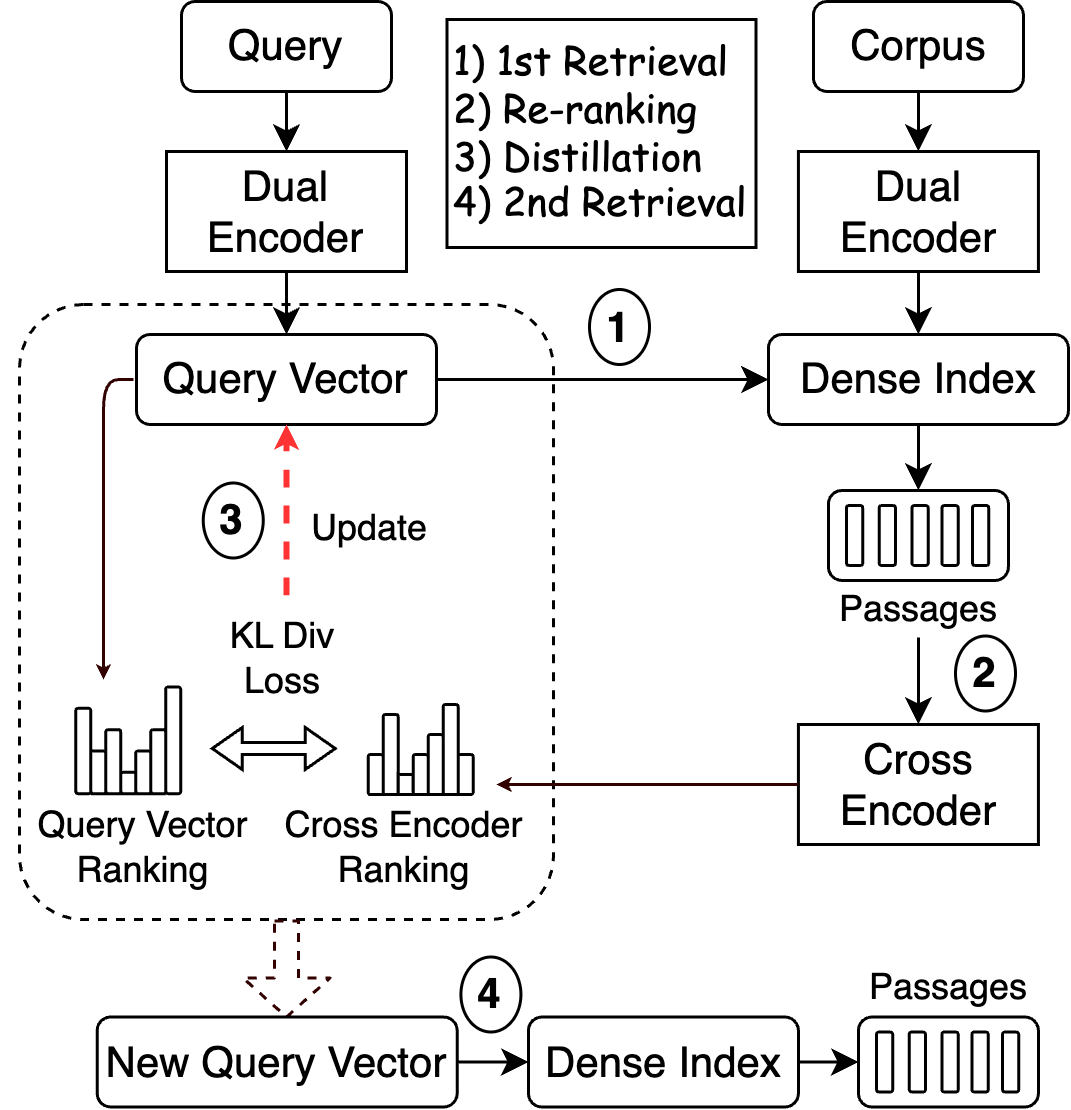
\includegraphics[width=1.0\linewidth]{submissions/Revanth2024/figures/cross_encoder_feedback_2.png}
    \caption{\textsc{ReFIT}: The proposed method for reranker relevance feedback. We introduce an inference-time distillation process (step 3) into the traditional retrieve-and-rerank framework (steps 1 and 2) to compute a new query vector, which improves recall when used for a second retrieval step (step 4).}
    \label{fig:overall_framework}
    \vspace{-1em}
\end{wrapfigure}

Since the more sophisticated reranker often generalizes better at passage scoring than the simpler, but more efficient retriever, here we propose to use relevance feedback from the former to improve the quality of query representations for the latter directly \textit{at inference}.
Concretely, after the R\&R pipeline is invoked for a test instance, we update the retriever's corresponding query vector by minimizing a distillation loss that brings its score distribution over the retrieved passages closer to that of the reranker.
The new query vector is then used to retrieve documents for the second time. 
This process effectively teaches the retriever how to rank passages like the reranker---a stronger model---for the given test instance.
Our approach, \textsc{ReFIT}\footnote{\textsc{ReFIT} stands for \textbf{Re}ranker \textbf{F}eedback at \textbf{I}nference \textbf{T}ime}, is lightweight as only the output query vectors (and no model parameters) are updated, ensuring comparable inference-time latency when incorporated into the R\&R framework. 
Figure \ref{fig:overall_framework} shows a schematic diagram of our approach, which introduces a distillation and a second retrieval step into the R\&R framework.
By operating exclusively in the representation space---as we only update the query vectors---our framework yields a parameter-free and architecture-agnostic solution, thereby providing flexibility along important application dimensions, e.g., the language, domain, and modality of retrieval. 
We empirically demonstrate this effect by showing improvements in retrieval on multiple English domains, across 26 languages in multilingual and cross-lingual settings, and in different modalities such as text and video retrieval.
 

Our main contributions are as follows:
\begin{itemize}
    \item We propose \textsc{ReFIT}, an inference-time mechanism to improve the recall of retrieval in IR using relevance feedback from a reranker.
    \item Empirically, \textsc{ReFIT} improves retrieval performance in multi-domain, multilingual, cross-lingual and multi-modal evaluation.
    \item The proposed distillation step is fast, considerably increasing recall without any loss in ranking performance over a standard R\&R pipeline with comparable latency.
\end{itemize}


